\hypertarget{the-kitaev-honeycomb-model}{%
\subsection{The Kitaev Honeycomb
Model}\label{the-kitaev-honeycomb-model}}

The Kitaev-Honeycomb model is remarkable because it was the first such
model that combined three key properties.

First, it is a plausible tight binding Hamiltonian. The form of the
Hamiltonian could be realised by a real material. Indeed candidate
materials such as \ce{\alpha-RuCl3} were quickly found
\cite{banerjeeProximateKitaevQuantum2016, trebstKitaevMaterials2022}
that are expected to behave according to the Kitaev with small
corrections.

Second, the Kitaev Honeycomb model is deeply interesting to modern
condensed matter theory. Its ground state is almost the canonical
example of the long sought after quantum spin liquid state. Its
excitations are anyons, particles that can only exist in two dimensions
that break the normal fermion/boson dichotomy. Anyons have been the
subject of much attention because, among other reasons, there are
proposals to braid them through space and time to achieve noise tolerant
quantum computations \cite{freedmanTopologicalQuantumComputation2003}.

Third and perhaps most importantly, it a rare many body interacting
quantum system that can be treated analytically. It is exactly solveable
meaning that we can explicitly write down its many body ground states in
terms of single particle
states\textasciitilde{}\cite{kitaevAnyonsExactlySolved2006}. Its
solubility comes about because the model has extensively many conserved
degrees of freedom that mediate the interactions between quantum degrees
of freedom.

To get down to brass tacks, the Kitaev Honeycomb model is a model of
interacting spin\(-1/2\)s on the vertices of a honeycomb lattice. Each
bond in the lattice is assigned a label \(\alpha \in \{ x, y, z\}\) and
that bond couples its two spin neighbours along the \(\alpha\) axis.

This gives us the Hamiltonian
\[\mathcal{H} =  - \sum_{\langle j,k\rangle_\alpha} J^{\alpha}\sigma_j^{\alpha}\sigma_k^{\alpha},\]
where \(\sigma^\alpha_j\) is a Pauli matrix acting on site \(j\),
(\langle j,k\rangle\_\alpha) is a pair of nearest-neighbour indices
connected by an \(\alpha\)-bond with exchange coupling
\(J^\alpha\)\textasciitilde{}\cite{kitaevAnyonsExactlySolved2006}.

\% plaquette operators and wilson loops This model has a set of
conserved quantities that, in the spin language, take the form of Wilson
loops \[W_p = \prod \sigma_j^{\alpha}\sigma_k^{\alpha}\] following any
closed path of the lattice. In this product each pair of spins appears
twice with two of the three bonds types, using the spin commutation
relations we can replace each pair with the third. For a single
hexagonal plaquette this looks like:
\[W_p = \sigma_1^{z}\sigma_2^{z} \sigma_2^{x}\sigma_3^{x} \sigma_3^{y}\sigma_4^{y} \sigma_4^{z}\sigma_5^{z} \sigma_5^{x}\sigma_6^{x} \sigma_6^{y}\sigma_1^{y}\]
\$\(W_p = \sigma_1^{x}\sigma_2^{y} \sigma_3^{z} \sigma_4^{x} \sigma_5^{y}\sigma_6^{z}\)
In this latter form can be seen to commute with all the terms in the
Hamiltonian because \{\color{red} why again?\}

The Hamiltonian commutes with the plaquette operators \(W_p\), products
of the \(K\)s around a plaquette. The Ks also commute with one another.
\[W_p = \prod_{<ij> \in P} K_{ij} = K_{12}K_{23}K_{34}K_{56} ... K_{N1}\]

Expanding the bond operators
\(K_{ij} = \sigma_i^{\alpha} \sigma_j^{\alpha}\), Pauli operators on
each site appear in adjacent pairs so can be replaced via
\(\sigma_i \sigma_j = \delta_{ij} + \epsilon_{ijk} \sigma_k\) giving a
product of Pauli matrices associated with the outward pointing bonds
from the plaquette. In the general case:
\[W_p = \prod_{i \in P} i (-1)^{c_i} \sigma_i\] where \(c_i = 0,1\)
measures the handedness of the edges around vertex i, see Fig
\ref{fig:handedness}. Plaquette operators for plaquettes with even
numbers of edges square to 1 and hence have eigenvalues \(\pm 1\), while
those around odd plaquettes have eigenvalues (\pm i) breaking chiral
symmetry. The values of the plaquette operators partition the Hilbert
space of the Hamiltonian into a set of flux sectors.

\% relationship between wilson loops and topology Such paths can enclose
a collection of faces or `plaquettes' of the lattice. In the case of
periodic boundary conditions, the system is torioidal and we also get
Wilson loops that wind the whole system without enclosing a definite
area. The loop operator associated with each such path has eigenvalues
\(/pm 1\) and can be interpreted as measuring the magnetic flux through
that region. Without going into the details of counting them, the number
of these conserved loop operators clearly scales with system size and it
is this extensive number of classical degrees of freedom that ultimately
allows us to decouple this interacting many body hamiltonian into a set
of non interaction quadratic hamiltonians. \{\color{red} add a figure
showing the different kinds of Wilson loops and of an example
plaquette\}

\begin{figure}
\hypertarget{fig:honeycomb_zoom}{%
\centering
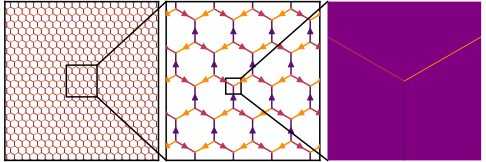
\includegraphics[width=0.5\textwidth,height=\textheight]{figure_code/amk_chapter/honeycomb_zoom/intro_figure_template}
\caption{\textbf{(a)} The standard Kitaev Model is defined on a
honeycomb lattice. The special feature of the honeycomb lattice that
makes the model solveable it is that each vertex is joined by exactly
three bonds i.e the lattice is trivalent. One of three labels is
assigned to each \textbf{(b)} We represent the antisymmetric gauge
degree of freedom \(u_{jk} = \pm 1\) with arrows that point in the
direction \(u_{jk} = +1\) \textbf{(c)} The majorana transformation can
be visualised as breaking each spin into four majoranas which then pair
along the bonds. The pairs of x,y and z majoranas become part of the
classical \(\mathbb{Z}_2\) gauge field \(u_{ij}\) leaving just a single
majorana \(c_i\) per site.}\label{fig:honeycomb_zoom}
}
\end{figure}

In order to actually solve the model we need to figure out how to
leverage these conserved quantities. The trick is not so much a trick as
an almost perfect consequence of the structure of the model and perhaps
this was in fact how Kitaev first came up with it. We know that a single
spin\(-1/2\) can be represented by fermionic creation and annihilation
operators \(\sigma^{\pm} = 1/2(\sigma^x \pm \sigma^y)\) through a
Jordan-Wigner transformation\textasciitilde{}\cite{}, this gives one
fermion for each spin. In turn a fermion can be broken into two Majorana
fermions \(c_1 = 1/\sqrt{1}(f + f^\dagger)\) and
\(c_2 = i/\sqrt{1}(f - f^\dagger)\). If we double up the Hilbert space
we get four Majoranas per spin:

\hypertarget{the-projector}{%
\subsection{The Projector}\label{the-projector}}

Closely following the derivation given in\textasciitilde{}\cite{} we can
extend the derivation of the projector to the amorphous case relatively
simply. The final form is {[}P\^{}0 = 1 + (-1)\^{}\{p\_x + p\_y + p\_z\}
\left(-i \prod\emph{\{\{i,j\}\} u}\{ij\}\right) \mathrm{det}(Q\^{}u) ;
\hat{\pi} {]} where (p\_x,p\_y,p\_z) are the parities of the
permutations required to reorder the (b\^{}\alpha\_i) operators into an
order where bonded sites are adjacent. These only depend on properties
of the amorphous lattice used. In the HLM these terms can be computed
analytically once a particular honeycomb lattice has been specified, we
instead compute then numerically using a fast cycle decomposition
algorithm.

(\mathrm{det}(Q\^{}u)) is the determinant of the matrix that takes
((c\_1, c\_2\ldots{} c\_\{2N\}) Q = (b\_1, b\_2\ldots{} b\_\{2N\})).
This along with (\prod u\_\{ij\}) depend on the lattice and the
particular vortex sector.

Finally (\hat{\pi} = \prod{i}\^{}\{N\} (1 - 2\hat{n}\_i)) is the parity
of the particular many body state determined by fermionic occupation
numbers (n\_i). The Hamiltonian is (H = \sum \epsilon\_i (n\_i - 1/2))
in this basis and this tells use that the ground state is either an
empty system with all (n\_i = 0) or a state with a single fermion in the
lowest level.

\subsection{Derivation}

The projector is just a product of the site projectors, let's say there
are (2N) sites. {[}D\_i = b\^{}x\_i b\^{}y\_i b\^{}z\_i c\_i {]} {[}P =
\prod\_i\^{}\{2N\} (1 + D\_i){]}

The clever trick from \ref{} is to note that this corresponds to a sum
over products of all possible subsets of the integers (the powerset) of
our 2N (D\_i) operators.

If we think of these subsets as bitstrings of length (2N) the we can
write this as a sum over integers (n) where (n\_i = 0,1) is the ith bit
of (n). {[}P = \sum\emph{\{n = 0\}\textsuperscript{\{2}\{2N\}\}
\prod}\{i=0\}\^{}\{2N\} D\_i\^{}\{n\_i\}{]}

then the ``all ones'\,' operator (F = \prod\emph{i D\_i) acts as the
bitwise not operation on any other subset: {[} \prod\emph{i D\_i
\prod}\{i=0\}\^{}\{2N\} D\_i\^{}\{n\_i\} = \prod}\{i=0\}\^{}\{2N\}
D\_i\^{}\{1 - n\_i\}{]} Hence we can actually just sum over half the
integers and use this operator to get the other half: {[}P =
\left(\sum\emph{\{n = 0\}\textsuperscript{\{2}\{2N - 1\}\}
\prod}\{i=0\}\^{}\{2N\} D\_i\^{}\{n\_i\} \right) (1 +
\prod\_\{i=0\}\^{}\{2N\} D\_i) = S P\^{}0{]}

The paper argues that S will never give zero on any state for reasons I
do not understand, though one can make an argument that since (P\^{}0)
already removes half the states from the Hilbert space, S cannot remove
anymore. We therefore focus on computing (P\^{}0).

{[}\prod\emph{\{i=1\}\^{}\{2N\} D\_i = b\^{}x\_1 b\^{}y\_1 b\^{}z\_1
c\_1; b\^{}x\_2 b\^{}y\_2 b\^{}z\_2 c\_2; \ldots{} ;b\^{}x}\{2N\}
b\^{}y\_\{2N\} b\^{}z\_\{2N\} c\_\{2N\}{]}

We can move all the (c\_i) operators to the right, incurring (3(i-1))
swaps for each giving a factor of (-1 \^{} \theta\_c) where ( \theta\_c
= \{3N(2N-1)\} = \sum{i = 1}\^{}\{2N\} 3(i-1))

{[}\prod\emph{\{i=1\}\^{}\{2N\} D\_i = -1\^{}\{\theta\emph{c\}b\^{}x\_1
b\^{}y\_1 b\^{}z\_1; b\^{}x\_2 b\^{}y\_2 b\^{}z\_2; \ldots{}
;b\^{}x}\{2N\} b\^{}y}\{2N\}
b\^{}z\_\{2N\};\prod\_\{i=1\}\^{}\{2N\}c\_i{]}

All the (b\^{}x) terms are separated by pair other operators so can be
brought to the front with no additional factors.

{[}\prod\emph{\{i=1\}\^{}\{2N\} D\_i =
-1\textsuperscript{\{\theta\emph{c\}\left(\prod}\{i=1\}}\{2N\}b\^{}x\_i\right)
b\^{}y\_1 b\^{}z\_1; b\^{}y\_2 b\^{}z\_2; \ldots{} ; b\^{}y}\{2N\}
b\^{}z\_\{2N\};\left(\prod\_\{i=1\}\^{}\{2N\}c\_i\right){]}

Finally we can send each (b\^{}z\_i) to the right incurring (i) swaps
giving (\theta\_z = N(2N - 1))

How to do open boundary conditions

Note: we don't actually compute (p\_x) we compute (-1ˆp\_x) directly
using a cycle decomposition to compute the permutation parity.

\subsection{Lattice generation}

\% diagram of a honeycomb lattice with majorana construction

\begin{figure}
    \centering
    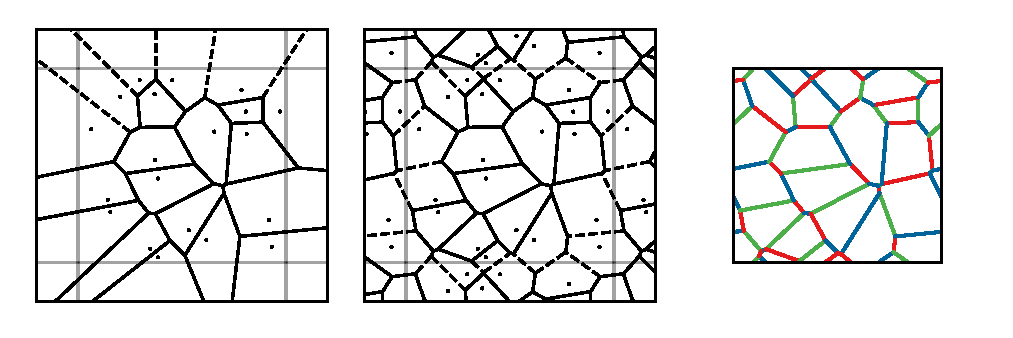
\includegraphics[width=\columnwidth]{figure_code/amk_chapter/lattice_construction/lattice_construction}
    \caption{\textbf{(a)}  \textbf{(b)}  \textbf{(c)} }
    \label{fig:honeycomb_zoom}
\end{figure}

We start from a set of points in the unit square. These can be drawn
uniformly or via other methods such as using blue-noise or jammed circle
packing.

We then tile the plane with images of the point in the unit square and
perform a voronisation over them. After this we can get rid of the
images and relabel edges that cross the boundaries (red lines in fig
\ref{fig:pbc_voronoi}) such that they connect points to the equivalent
point within the unit cell.

We represent the graph structure with an ordered list of edges ((i,j))
so we can represent both directed and undirected graphs which is useful
for defining the sign of bond operators (u\_\{ij\} = - u\_\{ji\}).

\% \subsetion{Kitaev-Heisenberg Model} \% In real materials there will
generally be an addtional small Heisenberg term \%
\textbackslash begin\{equation\} \% \label{eqn:kitaev_heisnberg} \%
\mathcal{H} = - \sum\emph{\{\langle j,k\rangle}\alpha\}
J\^{}\{\alpha\}\sigma\_j\^{}\{\alpha\}\sigma\_k\^{}\{\alpha\} +
\sigma\_j\sigma\_k \% \textbackslash end\{equation\}

\%

\section{The Projector} \label{apx:projector}

\% \{\color{red} Add brief mention of fermions and many body ground
state\} \% Closely following the derivation
of\textasciitilde{}\cite{pedrocchiPhysicalSolutionsKitaev2011} we can
extend to the amorphous case relatively simply. The main quantity needed
is the product of the local projectors (D\_i) \% {[}\prod\_i\^{}\{2N\}
D\_i = \prod\_i\^{}\{2N\} b\^{}x\_i b\^{}y\_i b\^{}z\_i c\_i {]} \% for
a lattice with (2N) vertices and (3N) edges. The operators can be
ordered by bond type without utilising any property of the lattice. \%
{[}\prod\_i\^{}\{2N\} D\_i = \prod\_i\^{}\{2N\} b\^{}x\_i
\prod\_i\^{}\{2N\} b\^{}y\_i \prod\_i\^{}\{2N\} b\^{}z\_i
\prod\_i\^{}\{2N\} c\_i{]} \% The product over (c\_i) operators reduces
to a determinant of the Q matrix and the fermion parity. The only
problem is to compute the factors (p\_x,p\_y,p\_z = \pm1) that arise
from reordering the b operators such that pairs of vertices linked by
the corresponding bonds are adjacent. \% {[}\prod\emph{i\^{}\{2N\}
b\^{}\alpha\emph{i = p}\alpha \prod}\{(i,j)\}b\^{}\alpha\_i
b\^{}\alpha\_j{]} \% This is simple the parity of the permutation from
one ordering to the other and can be computed easily with a cycle
decomposition.

\% The final form is almost identical to the honeycomb case with the
addition of the lattice structure factors (p\_x,p\_y,p\_z) \% {[}P\^{}0
= 1 + p\_x;p\_y;p\_z \mathrm{det}(Q\^{}u) ; \hat{\pi} ;
\prod\emph{\{\{i,j\}\} -iu}\{ij\}{]}

\% (\mathrm{det}(Q\^{}u)) is the determinant of the matrix that takes
((c\_1, c\_2\ldots{} c\_\{2N\}) Q = (b\_1, b\_2\ldots{} b\_\{2N\})).
This along with (\prod u\_\{ij\}) depend on the lattice and the
particular vortex sector.

\% (\hat{\pi} = \prod{i}\^{}\{N\} (1 - 2\hat{n}\_i)) is the parity of
the particular many body state determined by fermionic occupation
numbers (n\_i). The Hamiltonian is (H = \sum \epsilon\_i (n\_i - 1/2))
in this basis and this tells use that the ground state is either an
empty system with all (n\_i = 0) or a state with a single fermion in the
lowest level.

\begin{verbatim}
        Conserved quantities -> plaquettes
        Majorana representation with 4 per site
        Alternative representation with with 3 majoranas per site
        Mapping to BdG hamiltonian
        Vortex defects and lattice defects
        Kitaev on surfaces of genus g > 2
\end{verbatim}

Plaquette Operators Majorana representations 4 Majorana representation 3
Majorana representation

\subsection{Amorphous Models}
            \subsection{The Weire-Thorpe Model}

As a way to sanity check the code I was writing to work with the Kitaev
Honeycomb Model on Amorphous lattices it was useful to reproduce some
existing results.

\section{The Amorphous Kitaev Honeycomb Model}

Extending the kitaev honeycomb model to arbitrary trivalent lattices.
Even and Odd Plaquettes Degeneracy and euler's equation

\begin{figure}
    \centering
    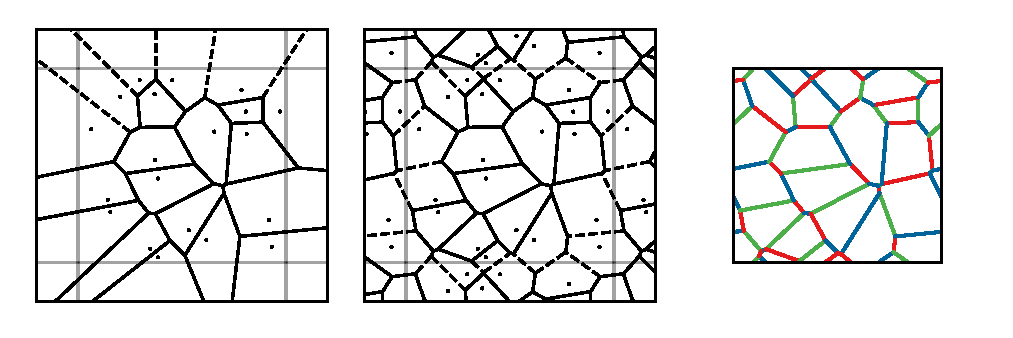
\includegraphics[width=\columnwidth]{figure_code/amk_chapter/lattice_construction/lattice_construction}
    \caption{\textbf{(a)} In-gap fermionic wavefunction drawn from the ground state flux sector in open boundary conditions, showing the state corresponds to a topological edge mode. Cut of the density along a line of lattice sites spanning the system (black line) is shown in the bottom subfigure on a logarithmic scale, demonstrating the characteristic exponential decay of topological edge modes with distance from the system edge. \textbf{(b)} Ground-state flux sector fermionic density of states in open boundary conditions, colored by inverse participation ratio. The increased inverse participation ratio of the in-gap states signifies their localisation to the edges of the system.}
    \label{fig:lattice_generation}
\end{figure}

\section{Methods}
        \subsection{Generating and Colouring Trivalent Graphs}
        \subsubsection{Voronisation}
        \subsubsection{Coloring}

The four colour theorem and its relation to edge colouring. Finding
Lattice colourings in practice: SAT solvers

\begin{verbatim}
    \subsection{Finding the Ground State Flux Sector}
        A* star on the graph
        Minimum spanning trees
\end{verbatim}

\section{Results}
    \subsection{The Ground State}
    \section{Ground State Phase Diagram}
    \subsection{The Flux Gap}

\section{Conclusion}
\section{Discussion}
\section{Future Work}

\section{The Kitaev Honeycomb Model}

\subsection{The spin model}

The Kitaev-Honeycomb model is an exactly solveable model of interacting
spins (or generic spin 1/2 degrees of freedom) on a honeycomb lattice.
The Honeycomb lattice is bipartite and trivalent (each vertex connects
to three others). The edges of the lattice are assigned to (x,y,z) such
that each site is connected to one of each type of edge.

{[}H = \sum\emph{\{\textless i,j\textgreater\}
J}\alpha \sigma\emph{i\^{}\{\alpha\} \sigma\emph{j\^{}\{\alpha\} =
\sum}\{\textless i,j\textgreater\} J}\alpha K\_\{ij\}{]} where (\alpha =
\alpha(i,j)) is the type of the bond linking sites i and j.

Various generalisations have been made, one mode replaces pairs of
hexagons with heptagons and pentagons
\cite{periNonAbelianChiralSpin2020} and another that replaces vertices
of the hexagons with triangles \cite{yaoExactChiralSpin2007}. When we
generalise this to the amorphous case, the key property that will remain
is that each vertex interacts with exactly three others via an x, y and
z edge. However the lattice will no longer be bipartite, breaking chiral
symmetry among other things.

The Hamiltonian commutes with the plaquette operators (W\_p), products
of the Ks around a plaquette. The Ks also commute with one another.
{[}W\_p = \prod\emph{\{ \in P\} K}\{ij\} =
K\_\{12\}K\_\{23\}K\_\{34\}K\_\{56\} \ldots{} K\_\{N1\}{]}

Expanding the bond operators (K\_\{ij\} = \sigma\_i\^{}\{\alpha\}
\sigma\_j\^{}\{\alpha\}), Pauli operators on each site appear in
adjacent pairs so can be replaced via (\sigma\emph{i \sigma\emph{j =
\delta}\{ij\} + \epsilon}\{ijk\} \sigma\emph{k) giving a product of
Pauli matrices associated with the outward pointing bonds from the
plaquette. In the general case: {[}W\_p = \prod}\{i \in P\} i
(-1)\^{}\{c\_i\} \sigma\_i{]} where (c\_i = 0,1) measures the handedness
of the edges around vertex i, see Fig \ref{fig:handedness}. Plaquette
operators for plaquettes with even numbers of edges square to 1 and
hence have eigenvalues (\pm 1), while those around odd plaquettes have
eigenvalues (\pm i) breaking chiral symmetry. The values of the
plaquette operators partition the Hilbert space of the Hamiltonian into
a set of flux sectors.

\% \textbackslash begin\{figure\} \% \centering \%
\includegraphics[width = 0.5\textwidth]{figs/vertex_handedness} \%

\caption{Plaquette operators defined as a clockwise product of bond operators will contain a term \(...K_{ki}K_{ij}... = ...\sigma^\alpha_i \sigma^\beta_i ...\) which can be replaced with \(i (-1)^{c_i} \sigma_i^\gamma\) where \(c_i = 1\) if the bond types going clockwise around vertex i are a cyclic permutation of xyz otherwise \(c_i = 0\)}

\% \label{fig:handedness} \% \textbackslash end\{figure\}

\subsection{A non-interacting Majorana representation}

The original Kitaev paper uses a transformation involving two fermionic
modes per lattices site: {[}\acomm{f^\dagger}{f} = 1, \acomm{f}{f} =
\acomm{f^\dagger}{f^\dagger} = 0{]} and the same for the second operator
(g). They anti-commute with each other and the operators on other sites.
It is also possible to transform to a Majorana basis with no redundant
degrees of freedom \cite{fengTopologicalCharacterizationQuantum2007}.

We also have the number operators (n\_f = f\^{}\dagger f) and the total
parity operator (P = (2n\_f - 1)(2n\_g - 1)) which divides the Hilbert
space into even ((\ket{00}, \ket{11})) and odd ((\ket{01}, \ket{10}))
parity subspaces.

The Majorana modes are defined by: {[}b\^{}x = f + f\^{}\dagger{]}
{[}b\^{}y = -i(f - f\^{}\dagger){]} {[}b\^{}z = g + g\^{}\dagger{]} {[}c
= -i(g - g\^{}\dagger){]}

Note that applying an odd number of Majorana operators to a state in one
parity subspace will flip it to the other, while any even number
preserves the parity subspace.

The Pauli operators live in a two dimensional Hilbert space. We can
build one from the fermionic subspace by projecting onto either the odd
or even parity subspace defined above. The parity can be easily defined
in terms of Majorana operators:

{[}D = b\^{}x b\^{}y b\^{}z c = - (2n\_f - 1)(2n\_g - 1) = - P{]}

And the Pauli operators can be defined w.r.t states with D = 1 :
{[}\sigma\^{}\alpha = i b\^{}\alpha c{]}

With this choice, the Hamiltonian becomes quadratic:

{[}H = \frac{i}{4} \sum\emph{\{\textless i,j\textgreater\} 2
J}\{\alpha\emph{\{ij\}\} u}\{ij\} c\_i c\_j{]} {[}u\_\{ij\} = i
b\^{}\{\alpha\_ij\}\_i b\^{}\{\alpha\_ij\}\_j{]}

\section{The Kitaev Honeycomb Model extended to an Amorphous Lattice}

\subsection{Edge Colouring}

\% \textbackslash begin\{figure\} \% \centering \%
\includegraphics[width = .5\textwidth]{figs/dual_graphs.png} \%

\caption{Two graphs which are dual of one another.}

\% \label{fig:dual_graphs} \% \textbackslash end\{figure\}

\% \textbackslash begin\{figure\} \% \centering \%
\includegraphics[width = \textwidth]{figs/k5} \%

\caption{Embedings of the complete graph \(K_5\) and its dual \(D(K_5)\) onto the torus. The vertices of \(K_5\) cannot be 4 coloured and the edges of \(D(K_5)\) cannot be 3 coloured.}

\% \label{fig:k5} \% \textbackslash end\{figure\}

Now that we have trivalent amorphous lattices, we need to assign
(\sigma\_x, \sigma\_y, \sigma\emph{z) to each edge. If we want the
Majorana transformation to remain useful then we require that each site
be connected to exactly on of each type of edge, otherwise the bond
operators (u}\{ij\}) would not commute with one another and the model
would not reduce to a quadratic form. This amounts to asking for a 3
coloring of the edges of the graph.

The famous 4 colouring theorem proves that the vertices of all planar
graphs can assigned one of four colors such that no neighbouring
vertices share a colour using 4 colors or more. This can be turned into
a proof that all trivalent planar graphs can be 3 edge coloured as
follows:

\begin{enumerate}
\def\labelenumi{\arabic{enumi})}
\item
  Define the dual of a graph G to be D(G) such that plaquettes of G
  become vertices of D(G) and neighbouring plaquettes sharing an edge in
  D(G). It's easy to see that if G is planar then so is D(G). Note that
  each edge in G corresponds to an edge in D(G) and each vertex of G is
  surrounded by a triangle of three vertices in D(G).
\item
  The vertices of D(G) can be 4 coloured with colors (a,b,c,d)
\item
  Assign a color from (i,j,k) to the edges of D(G) (and thus to the
  edges of G) according to the colors of the vertices linked by the
  edge, ignoring ordering:
\end{enumerate}

i if \{a,b\} or \{c,d\} j if \{a,c\} or \{b,d\} k if \{a,d\} or \{b,c\}

\begin{enumerate}
\def\labelenumi{\arabic{enumi})}
\setcounter{enumi}{3}
\tightlist
\item
  In a trivalent graph G, a vertex v in G is always part of 3 plaquettes
  (vertices in D(G)) and the colors of those plaquettes determines the
  colors of the edges that connect to v. The three vertices in D(G) must
  take three distinct colors from (a,b,c,d) so cannot lead to two edges
  with the same colour.
\end{enumerate}

This implies that all trivalent planar graphs can have their edges 3
coloured. However we work in periodic boundary conditions and it's easy
to embed the complete graph (K\_5) into periodic boundary conditions,
showing that the four colour theorem does not apply to periodic boundary
conditions. However numerically we have not yet encountered even one
case.

\% \textbackslash begin\{figure\} \% \centering \%
\includegraphics[width = \textwidth]{figs/edge_color} \%

\caption{On the left, a single vertex in G, and the three dual-vertices in its dual D(G). If the dual-vertices of D(G) are 4 colored, the three dual-vertices shown must be three distinct colors, and hence if the colors of the edges in G are chosen according to the rules on the right, each will be distinct.}

\% \label{fig:edge_color} \% \textbackslash end\{figure\}

\subsection{Finding Colourings}

Graph colouring is in NP, meaning that in general there is unlikely to
be a polynomial time algorithm to compute it. However that does not mean
that realistic instances of the problem are computationally intractable.
A common method in computer science is to map NP problems onto a
particular problem called Boolean Satisfiability for which general
purpose and highly optimised solvers have been written.

The problems can be written as a a series of statements about a set of
boolean variables, which we choose to be take to be the set
(l\_\{i\alpha\}) which indicate if edge i has colour (\alpha). We then
have two types of contraint: each edge is exactly on colour and no
neighbouring edges are the same color.

I'll fill in the encoding later but the gist is that we can give this to
a solver and get back: whether the problem is solveable, a solution or
all the possible solutions. Finding a solution is relatively fast, while
finding all the solutions is slower since there appear to be
exponentially many of them. Fig \ref{fig:multiple_colourings} shows some
examples.

\% \textbackslash begin\{figure\} \% \centering \%
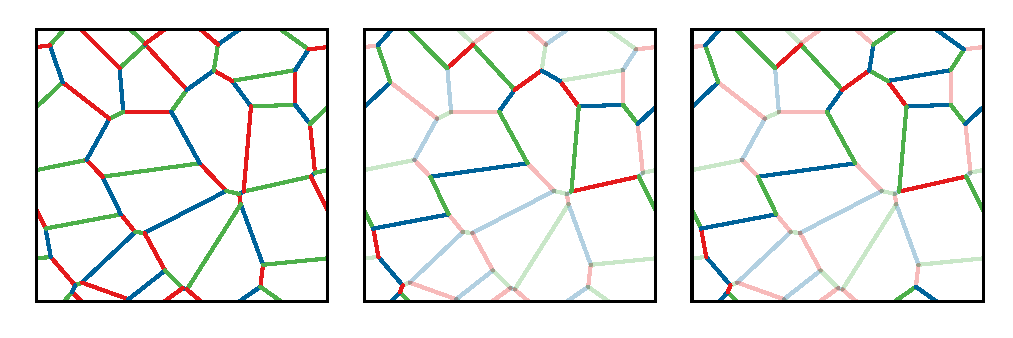
\includegraphics[width = \textwidth]{figs/multiple_colourings} \%

\caption{Multiple valid 3-edge-colourings of a random trivalent lattice. Edges are colored from red, green and blue and vertices are coloured red/blue if the edge colours are a cyclic/anticyclic permutation of rgb going clockwise around the vertex. Black edges or vertices indicate the color is the same as that in the top left. Note that some of the points are very close together, in future we will add a step to separate these.}

\% \label{fig:multiple_colourings} \% \textbackslash end\{figure\}

\section{Weaire-Thorpe Models}

As a benchmark for our graph algorithms we reproduce results on the
Weaire-Thorpe Model. The DOS agree very well but I haven't yet
understood how to plot the edge states, plotting a single state in the
gap or the sum of states in a finite energy region in the gap doesn't
seem to look like an edge state.

\% \textbackslash begin\{figure\} \% \centering \%
\includegraphics[width = \textwidth]{figs/WT_lattice} \%

\caption{An example of a Weaire-Thorpe model generated with our code.}

\% \label{fig:WT_lattice} \% \textbackslash end\{figure\}

\% \textbackslash begin\{figure\} \% \centering \%
\includegraphics[width = \textwidth]{figs/DOS_WT_Comp} \%

\caption{A comparison between the DOS from the paper (left) and the DOS generated using our code (right)}

\% \label{fig:DOS_WT_Comp} \% \textbackslash end\{figure\}

\section{Open Questions}
\begin{itemize}
    \item Are the excitation spectra of the flux sectors disparate or overlapping?
    \item Will there be a qualitative difference between choosing +i for all plaquettes of odd length and of choosing +/-i so that they cancel out?
    \item
\end{itemize}
